\chapter{Dark Sun Primer}

\begin{figure}[H]
\centering
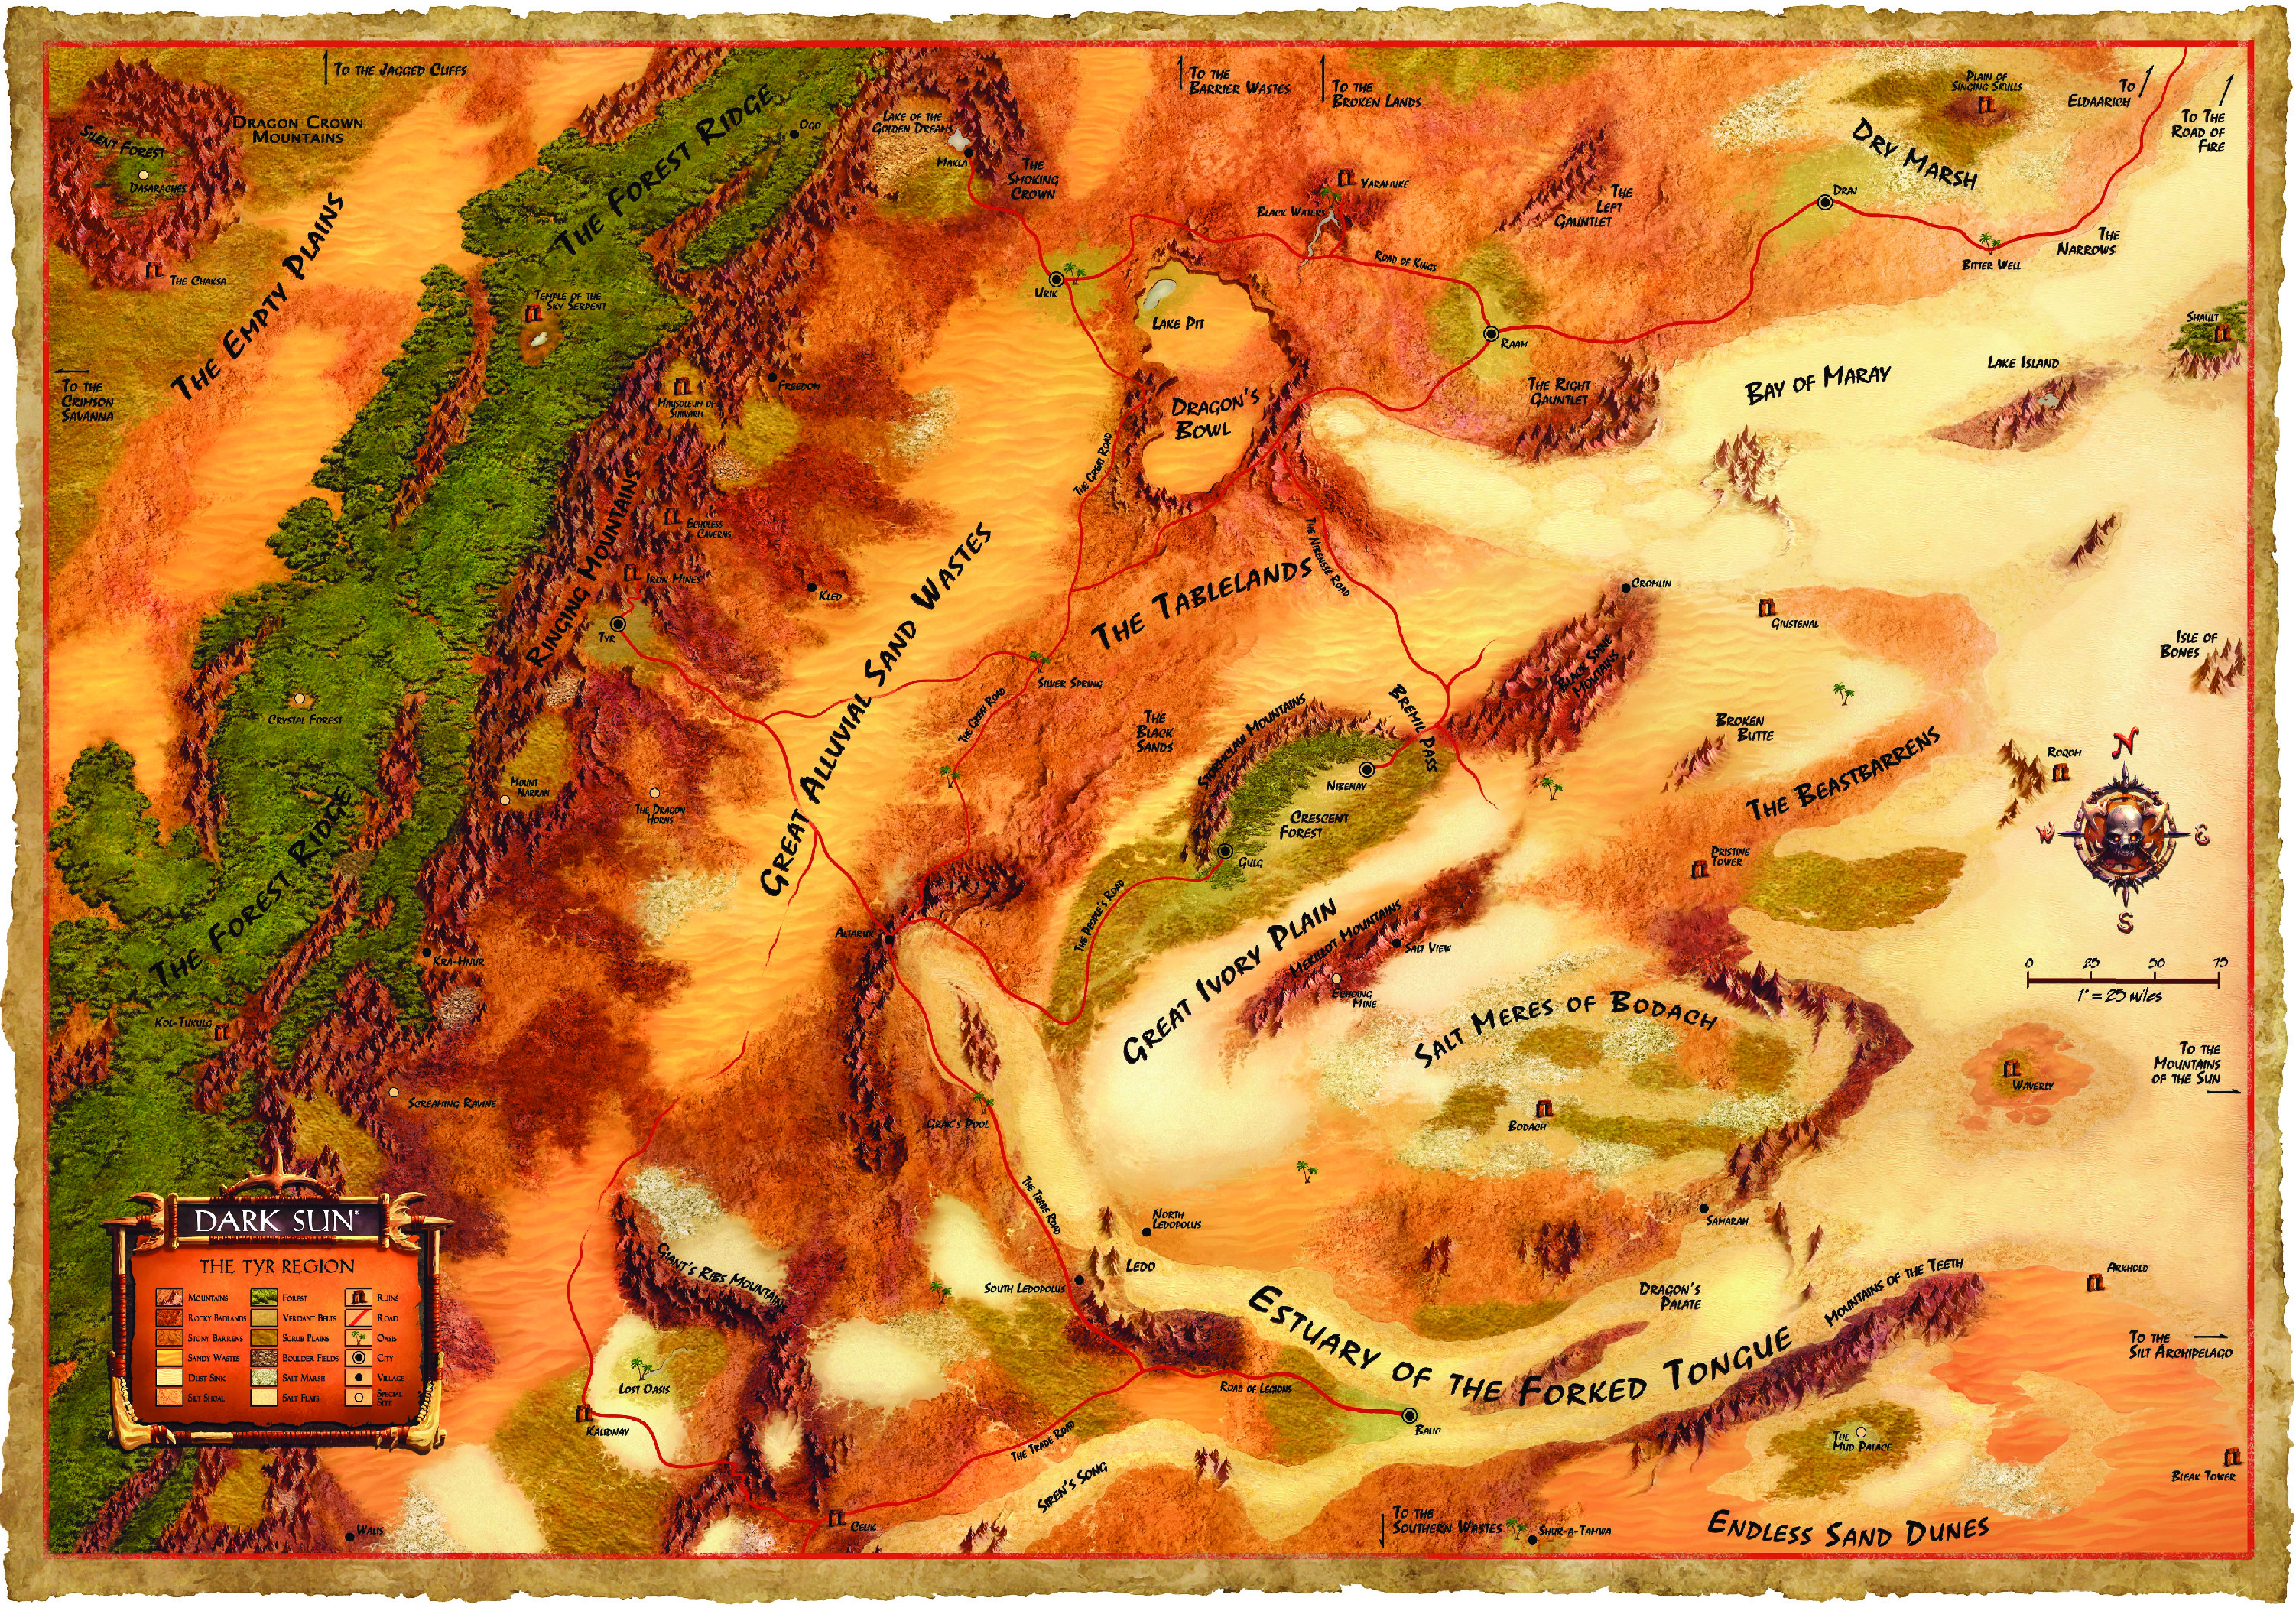
\includegraphics[width=0.98\linewidth]{images/world_map.jpg}
\end{figure}

\section{Life on Athas}

\epigraph{\textit{
"Almost all the Tyr Region is a desert wasteland, though it is beautiful and
spectacular in its own fashion. Over each hill, behind each sand dune, the
terrain appears more awesome than the land before. In my travels, I have
often been overwhelmed by the sheer magnitude of this land, cowed by its
indifferent brutality, even frightened by the unrestrained
might of its elements—but I have never been bored.\\
Can I impart the grandeur and majesty of this area with mere words? I
wonder. I can describe the queasy feeling of sliding down the glassy
slopes of the Smoking Crown, or make your eyes sting with tales of
walking the salt flats on a windy day. My words are but transparent
reflections of this magnificent land, but perhaps they can be of use." }}
{ The Wanderer’s Journal }

\begin{multicols}{2}

Athas is still a largely unknown world. Millennia of
misinformation, wars, and natural barriers have created
isolated pockets of civilization between large expanses of
desert terrain.\\
The known world is currently divided into the Silt
Sea, the Tablelands (also known as the Tyr Region), the
Ringing Mountains, and the Hinterlands. The Tyr Region
is defined as the area bordered by the Sea of Silt on the
east, the Hinterlands to the west, and the Endless Sand
Dunes to the south.\\
Outside of those regions, the Jagged Cliffs, the
Deadlands, and the Valley of the Cerulean Storm wait to
be discovered, charted, and plundered. The surface of
Athas stretches from horizon to horizon, a patchwork of
fields and forests, oceans (of water and sand) and
mountains, deserts, swamps, jungles, and more. Beneath
the crimson sun, Athas’ varied environments give way
one to another across the Tablelands. Mountains rise,
valleys fall, and desert surrounds the land.\\

\subsection{The World of Athas}
Athas is a desert‐sun‐scorched and wind‐scoured,
parched and endless, but that does not mean that the
landscape is monotonous. Far from it; over each hill,
behind each dune, the terrain is more awesome, more
spectacular, and more beautiful than any one has seen
before. North or south, east or west, Athas contains
natural wonders and dangers undreamed of on other
worlds.\\
\\
Storms blow in from the Sea of Silt, walls of pearly
dust billow ten thousand feet into the air, then come
roiling ashore like a mountain range crashing down about
unwary travelers. There are hundreds of different kinds
of terrain on Athas, from wind‐scoured pebble flats to
twisted badlands canyons to gleaming sands to jumbled
boulder fields.\\
\\
In this chapter, the world of Athas is examined from
the point of view of the Tablelands, also known as the Tyr
Region, the region that has influenced Athas (for good or
bad) the most.\\

\subsubsection{Tyr,The Free City}
\epigraph{\textit{
"Is it true? Kalak dead? Slaves freed? Magic wild in the
    streets? Doubtful, but we'll know soon enough."} }
{ Shahin, wandering hermit }

As far as most Athasians are concerned, Tyr has
always existed. Certainly it has endured through
the entire Desert Age, and even with the fall of its
sorcerer-king, it seems likely to endure for centuries
to come. And throughout all the long years of its exis-
tence, it was a city-state enslaved.\\
\\
That has all changed.\\
\\
In the courts of the other city-states, rumors of
King Kalak’s overthrow are only whispered, but in
Tyr, the repercussions howl through the streets. Many
scheme to succeed Kalak, and the templars and other
power groups vying for control struggle to keep the
city-state from disintegrating into anarchy at the
hands of people eager to enjoy their freedom. Nobles
and merchants clamor for influence, and commoners
and freed slaves openly celebrate, challenging civic
authority and social boundaries at every turn.\\

\subsubsection{Balic,City Of Sails}
\epigraph{\textit{
"In Balic, we treasure our freedoms. You are free to speak
as you will. Of course, Andropinis is also free to speak as he
will, which might very well be an order for your execution.
Choose your words with care, my friend."} }
{ Darian, a patrician of Balic }

A wealthy mercantile city-state on the shores of the
Estuary of the Forked Tongue, Balic is under the
control of Dictator Andropinis, a sorcerer-king who
claims to have been elected to his throne over seven
hundred years ago. Despite the dictator’s grip, Balic is
perhaps the most affluent city-state in the Tyr Region
and is home to powerful merchant houses that bring
great wealth to Balicans fortunate enough to share in
the prosperity. The business of Balic is business, and
for the most part, Andropinis does not interfere in
routine affairs of nobles or merchant emporiums.\\
\\
The city is renowned for its democratic traditions.
Balic’s nobles are seated in a Chamber of Patricians
that creates and maintains the code of laws, and its
templars must stand for election to 10-year terms.
The various professional guilds (and Balic’s chapter
of the Veiled Alliance, for that matter) conduct
their business by taking votes and electing officers;
even the dictator is, in theory, elected. Much of this
democracy, however, is little more than an illusion.
The office of dictator is held for life, and Andropi-
nis has endured in his position now for centuries.
Public debate and discourse is allowed, but only up
to a point. Any direct criticism of the dictator or his
templars is dealt with harshly, and the patricians
learned long ago to pass only those laws that meet
with the dictator's approval.\\
\\
Balic enjoys a cultural heritage and a civic
mythology dating back thousands of years, which
finds expression in a public appreciation for poetry
and drama. The mythology still lives in the form
of powerful arcane vestiges; Andropinis and his
templars are masters of manipulation. The cultural
heritage is evident in the dozens of theaters through-
out the city-state, which run the gamut from crowded,
ramshackle stagehouses in the poorer quarters to
magnificent amphitheaters in the noble districts.
In Balic, talented playwrights and orators can win
acclaim equal to that held by the greatest gladiators—
as long as they steer clear of subject matter that the
dictator’s templars might find offensive.\\

\subsubsection{Draj, City OF The Moons}
\epigraph{\textit{
"You, friend, have been given a great honor. To see the
Father is a rare blessing bestowed on only the worthiest
souls. What’s that you say? Sacrifice? Oh, yes-yes, indeed,
you will be sacrificed. Now don’t struggle so. To have your
heart claimed by a god—what a gift!"} }
{ Huemac, moon priest attendant }

Draj is a backwater city-state held firmly in the grasp
of a mad sorcerer-king. Draj has never known peace,
for warfare and conflict are among its highest ideals.
Warriors hold power, and their vaunted status is
something all aspire to attain. When not waging war
against Raam or defending their home from reprisals
or conquest, Draji raiders prowl the surrounding
wastes, plundering villages for fresh slaves to replace
those expended in labor or sacrifice.\\
\\
Draj owes its sinister nature to its sorcerer-king.
Tectuktitlay, the Father of Life, is a pervasive presence
in the city-state. His visage adorns walls and
buildings, his symbol ripples on banners, and his
templars (known as moon priests) are everywhere,
enforcing his laws and instructing the people in his
perfect divinity. No one would suggest it, but in fact,
the sorcerer-king’s features have little majesty.
Tectuktitlay has narrow eyes, a wide nose, heavy jowls,
and round, pouty lips. Other regal images include the
feathered serpent found on banners carried by soldiers
in war. The jasuan, or ambush drake, also has a
place of prominence in Draj.\\
\\
Tectuktitlay's influence is so insidious that most
Draji dare not question his divinity, doubt the deeds
attributed to him, or disobey the commands given
by his moon priests. All citizens know that dissent
invites the sorcerer-king's ire, and his anger can be
quelled only by blood sacrifice.\\

\subsubsection{Gulg,The Forest City}
\epigraph{\textit{
"You think you act in secret, but the forest ghosts see all that
occurs beneath their boughs. There are no secrets from the
Oba. She has sent me to show you the truth of this." }}
{ Chachak-Ke, judaga }

Many of the sorcerer-kings claim (or have claimed
in the past) to be gods upon Athas. In Gulg, that
assertion is made not by the sorcerer-queen of the
city-state but by its residents. Ask any Gulgan, and
he or she will tell you: Lalali-Puy, Queen of Gulg, is
the Oba, the Forest Goddess, the Mother of Trees
and Beasts, and a dozen more epithets besides. This
declaration is no empty platitude mouthed to avert
the baleful eye of the templars—the people of Gulg
sincerely believe that their ruler is divine.\\
\\
Gulg is a city only in the loosest definition of the
term; it consists of a cluster of forest villages enclosed
by a single wall. Most buildings are made of thatch or
mud, and roads are little more than trampled earth,
worn down by the feet of generations. Gulg is roughly
divided into small communities called dagadas,
each of which comprises ten to fifty huts. A dagada is
enclosed by a mud wall or wooden fence and is built
around one or more wells shared by the residents,
Lalali-Puy is an absolute monarch in the purest
sense: All property in Gulg is hers, and she holds the
ultimate power of life and death over all citizens,
from the lowest slave to the greatest judaga warrior.\\

\subsubsection{Nibenay,City Of Spires}
\epigraph{\textit{
"Raiders troubling the road to Raam? Unfortunate, I
suppose, but it hardly seems like cause for concern. Does
anything important come from Raam? Who would want
to go to Raam, anyway? If you must, send someone to bribe
some other band of savages to drive them off." }}
{ Sadag, Nibenese noble }

Ancient beyond measure, Nibenay is a wealthy, powerful
city-state immersed in decadence and intrigue.
Most Nibenese regard themselves as the only civilized
people remaining in a world of barbarism and
desolation; the events that take place outside the city
walls are little more than the squabbles of savages.
Even the architecture of Nibenay reflects these prejudices.
Splendid statues and carvings cover the walls,
public buildings, and private homes throughout the
city, depicting great heroes and honored ancestors
from ages long forgotten by the rest of Athas. Some
are works of surpassing beauty, some glorify ancient
triumphs, and others depict shocking hedonism.\\
\\
Nibenay is ruled by the sorcerer-king who gave
the city-state his name. He is an enigmatic, retiring
figure, rarely seen by anyone but his templars. Deep
within the royal compound at the city's heart - the
forbidden dominion called the Naggaramakam - 
Nibenay immerses himself in arcane studies and
mysterious pursuits, leaving governance to the
bureaucracy of his templars. He is so reclusive that
rumors of his death circulate every few years, giving
rise to unrest and feuding among the nobles until he
appears and puts to rest any stories of his demise.\\

\subsubsection{Raam,City Of Unrest}
\epigraph{\textit{
"Raam is a city exhausted. The land can support it no
longer. There are no treasures left to pluck from the earth.
The sorcerer-queen? She hides, knowing death waits in
every shadow. The warlords? Petty, feckless, and brutal.
Don’t waste your water on us." } }
{ Gaurav, disaffected rebel }

Ancient and magnificent, Raam has fallen far from its
formerly wondrous heights. Centuries of plundering
the countryside for its resources, rampant corruption
in its government, and the rule of a hedonistic
and disinterested sorcerer-queen have brought the
city-state to the brink of disintegration. The alabaster
quarries and gemstone mines stand exhausted;
reckless agricultural practices have led to disastrous
food shortages. In the streets, violent factions sworn
to one warlord or another battle for control as the
once-vibrant and influential city slips into ruin. Mobs
riot daily against their ineffectual ruler, the sorcerer-queen
Abalach-Re, and her templars dare not set foot
in some of the city's districts.\\
\\
The present difficulties might have been averted
by a strong hand, but Abalach-Re had less interest
in ruling than in feeding her insatiable appetite for
pleasure. Generations ago, she abandoned her royal
title and declared herself to be the representative of
an all-powerful deity known as Badna. Calling herself
the Grand Vizier, a title normally held by Raam's
greatest mystics, she razed the city's existing shrines
and temples, replacing them with new shrines dedicated
to Badna. The deity's image -that of a grinning,
four-armed male dressed in a long loincloth- appears
all over the city-state. Abalach-Re continues to assure
the citizens that Badna watches her closely and will
strike her dead if she falters in her duties, but few
believe her anymore.\\

\subsubsection{Urik,City Of Lions}
\epigraph{\textit{
"I am Hamanu, King of the World, King of the Mountains
and the Plains, King of Urik, for whom the roaring winds
and the mighty sun have decreed a destiny of heroism, and
to whom the life-giving waters and nourishing soils have
entrusted the mightiest city of Athas." }}
{ Hamanu, King of Urik }

Hamanu boasts with good reason. Urik is a powerful
city-state with teeming armies, enormous walls,
bustling commerce, and wise sages, governed in an
orderly framework established by the self-styled King
of the World. Urik's legions have never met defeat,
and Hamanu has never run from battle. Any decision
of importance made in the Tyr Region must consider
the wishes of Urik’s sorcerer-king.\\
\\
Urik is highly organized and militarized. A variety
of laws contained in the lengthy document known as
Hamanu's Code govern commerce and taxes, specify
holidays, set standards for construction and artistry,
and dictate family arrangements such as weddings,
care for elders, and funerals. Templars test Urikite
children and assign them to the vocations for which
they are most suited. The city aspires to be a meritocracy,
but hidden webs of patronage and influence
secure important posts and stations for people with
the right connections.\\
\\
Although Urik seems stable and well-ordered, it
is every bit as oppressive as any other city-state — perhaps
more so, thanks to the number and efficiency
of Hamanu's templars. In recent weeks, the fall of
Kalak of Tyr has upset Hamanu's delicate balance by
proving that sorcerer-kings who rule for centuries
might be mortal after all. Hamanu believes that he
has nothing to fear from his subjects, but he knows
that Urik's fortunes depend on trade with other cities.
If unrest spreads beyond Tyr, even Urik might suffer.
Thus, Hamanu’s templars keep an eye on developments
in the Free City and pay for information from
spies in Tyr, including the mul stonecutter Xalos.\\

\end{multicols}

\hrulefill

\subsection{Organizations}

\epigraph{\textit{
"Traders cooperate for Profit. Templars form allegiances for Domination. Psions join schools to gain Knowledge. And
raiders band together for Strength. Power comes in many forms, but all who band together seek it - intentionally or
unknowingly. Those who join them are caught in a web, for all organizations are tainted with corruption. The Veiled
Alliance seeks to overthrow the Sorcerer-Kings and justifies murder in its ranks out of fear for discovery. The elitist Order
would deny all other beings the use of psionic power and drive tens of thousands of beings insane. And the first generation
dray believe they are children of a god, who has banished them from their homes. Once you realize the secrets of your
organization, it is too late, for you are shackled to it. You realize you have traded your freedom for power." } }
{ The Oracle, Blue Shrine Scrolls }

\begin{multicols}{2}

In a Dark Sun campaign, characters may have to deal
with intrigue and sabotage as often as with creatures of
the Athasian wastelands. The descriptions that follow
represent only a few of the many organizations that
operate across the Tablelands and beyond. Some can be
used as patrons for adventurers, other as opponents.
More often, these organizations can be an ally one day,
and opponent the next.

\subsubsection{The Brotherhood of the Mind}
\epigraph{\textit{
"I am not sure what happened, but over what seems to be
the course of a month, this newcomer upstart became the
heir of the house. I have never heard of him in all my
travels across the Tablelands. I do not trust this Lergit
Mylor." }}
{ Polutick Fest of House Stel on the declaration of a
  new heir and secret member of the Brotherhood of the Mind }

The Brotherhood of the Mind is an ancient society of
evil psionicists that conspire to destroy all sorcerer‐kings
and rule Athas supreme. In the Sanctuary, they secretly
plot and scheme while constantly searching for ancient
psionic texts.

\paragraph{Brief History}
The Brotherhood was founded by a noble Nibenese
psionicist named Liumakh almost 500 years ago. Liumakh
is a powerful telepath who dreamed of unseating the
Shadow King of Nibenay. He was convinced that a
sufficient gathering of psionic power could defeat the
tyrant. Unfortunately, the Shadow King learned of his
plots, and he and his followers were forced to flee. At that
time, Hamanu of Urik was feuding with Nibenay, and he
gave them sanctuary.\\
\\
Liumakh and his followers constantly work to bring
down the Shadow King, but they've never been able to
succeed. In studying his enemy, Liumakh realized the
nature of the sorcerer‐kings, and his secret order changed
its goal to the accumulation of raw power. He planned to
destroy the sorcerer‐kings and assume his role as the ruler
of Athas.\\
\\
Over the centuries, the Brotherhood's importance has
fluctuated. Despite this, not one sorcerer‐king has fallen to
its plots. The Order closely watches the Brotherhood, but
to date it has not achieved a level of power that would
require intervention. Hamanu of Urik pretends to ignore
them, but he occasionally spies on the Brotherhood to see
what they are up to.\\
\\
The Brotherhood has taken advantage of the recent
events that shook the Tablelands, falsely advertising that
the sorcerer‐king of Tyr was killed by
members of the Brotherhood, which has caused their
ranks to substantially grow in the last few years. The
insulation of Urik has further helped the Brotherhood to
further grow, since now they are unfettered by Hamanu's
templars.\\
\\
\paragraph{The Brotherhood on Athas}
\epigraph{\textit{
"The sorcerer-kings are like large beasts, they go where you
lead them. Hunting large animals is always about choosing
the right battle ground, and one never attacks a drake in
its lair." }}
{ Liumakh, Leader of the Brotherhood }

The Brotherhood of the Mind is a secretive and
somewhat large body of evil manifesters, spreading out
into Athas searching for more members and ancient
psionic mysteries.\\
\\
The Brotherhood is a network of likeminded
individuals, all committed to advancement of their craft
and power. Although most train at the Sanctuary, only a
few members remain there. Most leave, returning on
occasion to share information, learn new powers, or seek
an audience with Liumakh.\\
\\
Officially, members are free to come and go as they
please, but in reality, any ex‐member will suffer a terrible,
fatal accident soon after leaving the Brotherhood. After all
it is a steep climb down. Liumakh is afraid that ex‐
members could reveal any important information to the
sorcerer‐kings.\\
\\

\subsubsection{The Dynastic Merchant Houses}
\epigraph{\textit{
"Sometimes, I don’t know whether to praise them or curse
them. They live in my city, they take up valuable space
and resources, and yet they obey me only when it suits
them. They say that they wish to maintain the general
good, keep things stable so that they may make a profit.
And yet, without them, my people would be unable to raise
great monuments to my glory, or perhaps even to eat! And
should my people grow dissatisfied, they would not submit
so easily to my rule, and would not give me the honor and
reverence I deserve. These traders are a pain, but what
would I do without them?" }}
{ Kalak the Tyrant of Tyr }

The merchant houses supply the lifeblood of
Athas―foodstuffs that feed isolated city‐states,
construction materials to build the palaces of sorcerer‐
kings and decadent nobles, slaves to toil in fields or fight
and die in gladiator pits, and many other vital items.
For specific information regarding an individual
Dynastic Merchant House refer to the Trader Lords
supplement.

Organized along family lines with a matriarch or
patriarch at its head, a major house controls dozens of
caravans, maintains estates in several different cities,
sponsors trading villages, and employs (or owns)
thousands. The largest houses―Wavir, Tsalaxa, and their
ilk―are influential enough to make even the most
powerful sorcerer‐kings take heed.

\subsubsection{The Order}
\epigraph{\textit{
"We are the Order, Ardivan the Black, and you will join
us in upholding the Balance or be destroyed." }}
{ Sashaya, female half‐elven entrant of the Order }

The Order is an organization of the highest‐level
psions on Athas, dedicated to two precepts: Psionics
should only be studied for its own sake, and psionic
talents should only be used to preserve the natural order.
To members of the Order, psionics is not merely a tool
or a means towards an end. Psionics is a higher
understanding, an area of study that purifies the mind
and strengthens the spirit. A purist of the Order believes
that he gains more awareness of the universe with every
new power he masters, with every new iota of psionic
strength that he can muster.\\
\\
In the doctrine of the order, psionics is a part of the
natural order, used by animals and primitives to survive
against the harsh environment and against each other.
Animals have retained this philosophy, but intelligent
races have perverted psionics, polarizing it along with
their moralities. Nature knows no such moralities. To a
member of the Order, ambitions and ideals can only
interfere with the purity o psionics. The use of psionics to
further such ambitions, whether good or evil, is a crime
against the natural order. Psions who use their talents to
further causes of extreme good or extreme evil are
criminals who must be located and stopped.\\

\paragraph{Brief History}
The history of the Order is shrouded in mystery and
myth. Most of those who know of the Order only know of
their involvement in what has been named the Dragon’s
Crown incident, in which all psionic ability was
suppressed for a period of months in Mountain’s Fury of
the 190th King’s Age or Free Year 4.\\
\\
This incident began when the human psionicist
Pharistes became the Cerebral Master of Telepathy. It is
believed he blamed the wanton abuse of psionic power
for personal gain as the principle reason for the current
state of Athas. At some time in the past, Pharistes had
come into possession of an artifact called the Psionatrix
which was capable of suppressing psionic use.\\
\\
Once he became a Cerebral Master of the Order,
Pharistes presented his plan to correct the world to the
other Cerebral Masters. Using the Psionatrix, psionic
power would be suppressed across all of Athas for a
thousand years. During this time, the Order would set
things rights, as members were somehow immune to the
effects of the artifact. Though some of the Cerebral
Masters objected to this plan Pharistes was able to seize
control of the group through his superior telepathic
abilities and the power of the Psionatrix.\\
\\
The Psionatrix was activated and a psionic
suppression field covered the planet. Chaos ensued.
Psionics is an integral part of Athasian life and used for
many mundane tasks through the day. The disruption of
psionics caused considerable damage to the cities of the
Tablelands. In addition, the psionic suppression field had
a side effect on thri‐kreen, causing them to enter a berserk
uncontrollable rage.\\
\\
According to rumors, King Hamanu eventually
discovered the location of Pharistes and the Psionatrix in
an ancient fortress deep in the Dragon’s Crown
Mountains. The Lion King sent agents to deactivate the
Psionatrix. Apparently the heroes succeeded thought
rumors vary on whether Pharistes was killed or driven
off, and what became of the Psionatrix.
In the aftermath of the Dragon’s Crown incident
rumors spread that the Order was left in turmoil. Their
agenda and methods questions with many members
questioning whether the Order should continue as an
organization or disband. In recent years, rumors that the
Order has disbanded have been passed by those in the
known. With the battle at the Dragon Crown Mountains
having significantly reduced their numbers and a
disagreement over whether the Order should reconsider
its goals, the members decided to disband the remnants of
the Order.\\

\paragraph{The Order on Athas}
\epigraph{\textit{
"Psionic heresy cannot be allowed. By our ancient laws he
is now a renegade. His life is forfeit." }}
{ Mandalis, Order Mediator }

The Order is a self‐appointed champion of psionic
purity. The upper orders pursue psionic purity, whereas
lower orders root out heretical psions.\\
\\
The Order defines psionic heresy as the use of
powerful psionic powers for causes of extreme good or
evil. Powerful psionics are powers used by an epic psion.
Below that level, the Order regards psions as hardly more
than children, who cannot be held responsible for their
actions. The attitudes of such low‐level characters
towards law or chaos do not concern the Order.\\
\\
Characters who use other powers, (armies or arcane
magic, etc.) to further their good or evil ends also do not
concern the Order. Only the use of powerful psionics
draws the Order’s attention. The Order is not interested in
supporting neutrality as such‐they only seek psionic
purity as they have defined it.\\
\\
All members of the Order must uphold this agenda.
They must confront heresy according to their roles; they
must pursue greater psionic mastery themselves, and they
cannot personally use their psionic powers for any
purpose that is completely good or evil.

\subsubsection{The Shadows}
\epigraph{\textit{
“You might as well try to hide treasure from the
Shadows.” }}
{ Athasian proverb meaning something impossible }

Many Athasian organizations trade in contraband,
assassination, espionage and forbidden items—even, on
occasion, the dynastic merchant houses. But no others
have honed the practices of smuggling and trade in illegal
objects and substances to such a height as have the
Shadows, and no one knows exactly how they do it.

\paragraph{Brief History}
Many Athasians claim that the Shadows have always
existed. There is little evidence to contradict this, for
references to the Shadows go back hundreds of years.
After so much time, the Shadows have evolved
considerably, becoming less a tribe or family and more a
vast, complicated secret society with an exclusively elven
membership. While most Shadows are born into the
group, outsiders are sometimes admitted.\\
\\
An early reference to the Shadows comes from an
ancient epic sung by bards. This is known as "The Saga of
the Fall of Kaday". The song speaks of Kaday, a powerful
defiler, who is undone by a jealous ex‐lover. Spurned and
rejected, a beautiful wizardess makes a pact with a
mysterious group of black‐clad elves, giving them all her
worldly possessions in order to grant her vengeance. To
her dismay, the elves retaliate out of all proportion,
casting down Kaday in a cataclysm that destroys both
him and everything he owns. In the end, the distraught
wizardess repents of her deed and dies of grief.\\
\\
This story, a popular tragedy told in innumerable
versions (in one, the rejected wizardess and her lover still
wander the wilderness of Athas, wailing endlessly),
illustrates several points that are familiar to those who
know the Shadows. An inherent (if chaotic) sense of
justice and fair play seems to permeate their dealings.
Orders are often followed to the letter, even to the extent
of causing destruction and grief far out of proportion to
what the client initially requested. The Shadows, it seems,
are determined to teach foolish outsiders to think about
the consequences of their actions.\\
\\
Every city, as well as most villages, has tales about the
Shadows. They can take the role of heroes, villains, or an
amoral force of nature. Sometimes, they are thieves who
can be foiled only by the quick thinking of brave templars.
At other times, the Shadows are noble avengers who
frustrate the goals of greedy sorcerer‐kings or brutal
bandits. In all the stories they are similar—dark‐clad, soft‐
spoken elves who provide any service or obtain any item,
for a price.

\subsubsection{The Templarate}
\epigraph{\textit{
"Do you know the penalty for trying to escape the Shadow
King’s slave pits, my thin, elven captive?" }}
{ Alethea, Nibenese templar }

Templars are the minions of the sorcerer‐kings; his
warriors, his city‐guard, and the living symbols of his
tyranny.

\paragraph{Brief History}
The templars are taught that long ago the sorcerer‐
kings banished all gods as false and sent hordes of selfish
and misguided followers packing. Some believe this to be
true, and others say it is only a convenient lie created to
justify the Eradication. The majority of templars don’t
really care. They care more for the power they have and
with scheming to acquire more.
\paragraph{The Templarate on Athas}
\epigraph{\textit{
"Templars so cherish their status as keepers of the peace
and protectors of the public that they have occasionally been
known to beat to death those citizens who question that
status." }}
{ Wanderer's Journal }

The templarate is one of the great powers of the
Tablelands. Thanks to its control over a particular city‐
state administration and the divine spells granted by their
sorcerer‐kings, it has exerted considerable influence over
the shape of their city‐state during the Brown Age.
Characters who serve the templarate as templars or
templar knights are part of a significant and vital city‐
state power.

\subsubsection{The Veiled Alliance}
\epigraph{\textit{
"We hunt down the hidden cowards because they can't be
trusted. Only those chosen by the God-King Hamanu are
worthy of wielding the power of the mage. Only they are
controlled enough not to turn what precious little life on
Athas is left into dust and ashes." }}
{ Templar Distry Kentus, leader of Hamanu's anti‐wizard force }

In most cities, there are secret leagues of preservers
called the Veiled Alliance. The Veiled Alliances are
confederations of preservers working together to protect
their members from assassination and harassment by
sorcerer‐kings and other lieges. The members work
together to shield each other’s identities from the
authorities or to help those who have been discovered to
escape persecution and are often involved in plots to
overthrow their oppressive overlords.

\paragraph{Brief History}
It wasn’t long after the first battles of the Cleansing
Wars scoured the face of Athas that the common people
learned to fear all types of magic. This fear soon became a
burning hatred, and that hatred was directed at wizards
and suspected wizards in the villages and towns across
the land. The fear and hysteria caused by the wars incited
mobs to attack wizards-defilers and preservers both-
who were seen casting magic of any kind. Accusations of
wizardry spread quickly, and many folk without any sort
of magical skills were killed due to ignorance, false
accusations, or malicious lies. Many good wizards, whose
only crime lay in trying to help their people, also perished
at the hands of hysterical mobs.\\
\\
To protect themselves against the crowds and the
armies of the Champions, wizards learned to hide
themselves and their art. Defilers usually chose the road
of solitary study, while some preservers formed into
hidden groups. These preserver groups were opposed to
defilers, and especially to the Champions of Rajaat. They
bided their time, learning new magic, becoming stronger,
and searching for those who had the ability to learn the
ways of the preservers. The traditions of secrecy and
underground rebellion were thus set in motion thousands
of years ago, eventually evolving into the organization
known as the Veiled Alliance once the Brown Age began.

\paragraph{The Veiled Alliance on Athas}
\epigraph{\textit{
"We wear the veil to hide our identity, both from the
enemy who destroys the land, and from the common folk,
who we work to protect. Neither understands us. The
world of yesterday was a verdant paradise, and it can
return once we tear down the rulers of the city-states and
their templars."}}
{ Yang'til Urgrant to his new apprentice }

Sorcerer‐kings send their agents to destroy potential
rival wizards hiding within their cities. Nomad witch‐
lords banish rival mages to the unforgiving sands of the
desert. Halfling chiefs exterminate followers who show
any sign of control over the supernatural. Even otherwise
timid hermits have been known to risk their lives in an
effort to make sure that no wizard enters their territory.
The Veiled Alliance is an excellent nemesis or
potential ally for campaigns featuring arcane casters.
Veiled ones can act as tutors and suppliers or as recurring
foes, harrying PCs if they have an affiliation with defiling
magic or the sorcerer‐monarchs.

\subsubsection{Slave Tribes}
\epigraph{\textit{
"Slave tribes vary based on who their leader is. Most tribes
settle away from cities, and seek to stay hidden, avoiding
slavers and their former masters. They rarely trust
outsiders, and I have been attacked on more than one
occasion by those whom I came too close to." }}
{ Wanderer's Chronicle }

When a slave manages to escape, he must find his way
to one of the slave villages dotting Athas or perish in the
harsh wilderness. Usually, these villages serve as the base
for a raiding tribe, for slaves seldom have the skills
necessary to survive in the desert.\\
\\
The attention of a slave tribe is primarily directed at
the city‐states themselves, as well as the caravans carrying
goods between those city‐states. In this regard, their
violence can be excused, for it almost takes on the
character of a war against their former masters. In fact,
slave tribes have been known to attack templar caravans
and expeditions at great risk to themselves-even when
there was no economic incentive.\\
\\
Slave tribes tend to have a wide variety of races. In
every city‐state, a wide selection of races is used as slaves.
An equally wide selection escapes and finds its way to the
slave villages, so it should come as no surprise to discover
that most slave tribes are composed of a wide variety of
races.\\
\\
\paragraph{Slave Tribes on Athas}
\epigraph{\textit{
"They are a strange lot, banding together out of need and
hope. They settle just when they have gained freedom,
putting down roots when they have finally felt the wind on
their faces." }}
{ Gldarith Cloudracer of the Sky Singers tribe }

Slavery exists throughout Athas. It thrives in the city‐
states of the sorcerer‐kings. It flourishes in the merchant
houses. It lingers in villages far from the centers of
civilization. Almost every living, intelligent being knows
of the practice of capturing, raising, and keeping slaves.
Some relish the system and embrace its methods and
ideology completely.\\
\\
Slave tribes are the most relief from the harsh and
cruel life an Athasian can dream of. A slave tribe can
represent a safe haven for procured PCs, since most slave
tribes are located in remote and easy to defend locations
or simply a rest stop for tired adventurers.

\subsubsection{Raiding Tribes}
\epigraph{\textit{
"They are a scourge, and should be wiped out. They ride
in, their leader with his foolish iron helm, and terrorize
honest traders, taking what they will. It costs more to
avoid the area, but we make up for it with less cargo lost." }}
{ Merchant Kel'lich of House Vorr about the Black }

Others living in the wastes beyond the city‐states
engage in very hostile approaches to earning a living.
These groups become raiding tribes, procuring what they
need to survive by pillaging caravans, poaching herds,
and plundering weak villages. Cutthroats, thieves,
murderers, and raiders hide in the desolate salt flats or
among the canyons of the rocky badlands, emerging only
long enough to strike before running back to their hole
with whatever spoils they can carry.\\
\\
Although raiders may be scoundrels and cutthroats,
they are not fools. They do not prey upon those who
stand a chance of fighting back and winning. Tribes
numbering no more than one or two dozen prey upon
hermits and small parties of travelers. On the other hand,
the tribes that plunder caravans number in the hundreds
and those that loot villages have as many as a thousand
members.\\
\\
Most raiders make their homes in some forlorn place,
such as rocky badlands or a secret oasis in the middle of a
salt plain. Of course, the raiders are attempting to hide
their location, but the isolation of their villages also makes
it difficult and expensive to send a force to destroy them.
This tactic works all too well; I can count on my fingers
the number of raiding tribes that I know to have been
destroyed in retribution for their thievery.\\
\\
Usually, the raiding tribes pick their leaders through a
hierarchy of violence. The most deadly (often a defiler) is
the leader. Invariably, he chooses the most dangerous and
toughest tribe members as his assistants, ensuring their
loyalty through special rewards and treatment. The other
members of the tribe are kept in line through the threat of
force. If the leader is a wizard, he will seldom tolerate the
presence of another wizard in his tribe. If the leader is not
a wizard, one of his assistants is usually a defiler who
jealously guards his position in the tribe.

\end{multicols}
